\documentclass[12pt]{article}
\usepackage[backend=bibtex,style=ieee]{biblatex} 
\addbibresource{mybib.bib}
\usepackage[margin=2.54cm]{geometry}
\usepackage{amsmath} % For equations of more than one line
\usepackage{sectsty} % Customise headings
\sectionfont{\centering\MakeUppercase}
% Side by side images
\usepackage{graphicx}
\graphicspath{ {./images/} }
\usepackage{caption}
\usepackage{subcaption}

\usepackage[section]{placeins} % Ensure that images go in the right section



\title{Transfer learning in mammography}
\author{
W Murphy
}
\date{\today}


\begin{document}
\maketitle

\begin{abstract}
This is the paper's abstract \ldots
\end{abstract}

\section{Introduction}
When data for training complex neural network is limited, (thousands oppose to millions of images) transfer learning becomes a necessary tool.  Transfer learning is the process of taking a network that has been trained on a large dataset, such as ImageNet, and retraining only the final layer on a new dataset.  

This technique has the potential for far more complex networks to be trained on a small dataset of mammograms and achieve high classification accuracies. 


\section{Methodology and preliminary results}
\subsection{Pre processing the images}
The dataset is comprised of 2980 DICOM images where 1489 are mammograms which are malginant (contain a cancer) and 1490 which are of a healthy breast (not cancerous).  The DICOM image format is the international standard to transmit, store, retrieve, print, process and display medical imaging information \autocite{dicom}.

The images are large and varying in size, around 2000 by 3000 pixels, 13 bit grey scale.  Before using the images to train a neural network, the ROI (region of interest) coordinates will be found so that they can be cropped to a much smaller size (200 by 200 pixels) with the cancer, if apparent, centred in the image.  

\begin{figure}
\centering
\begin{subfigure}{.5\textwidth}
  \centering
  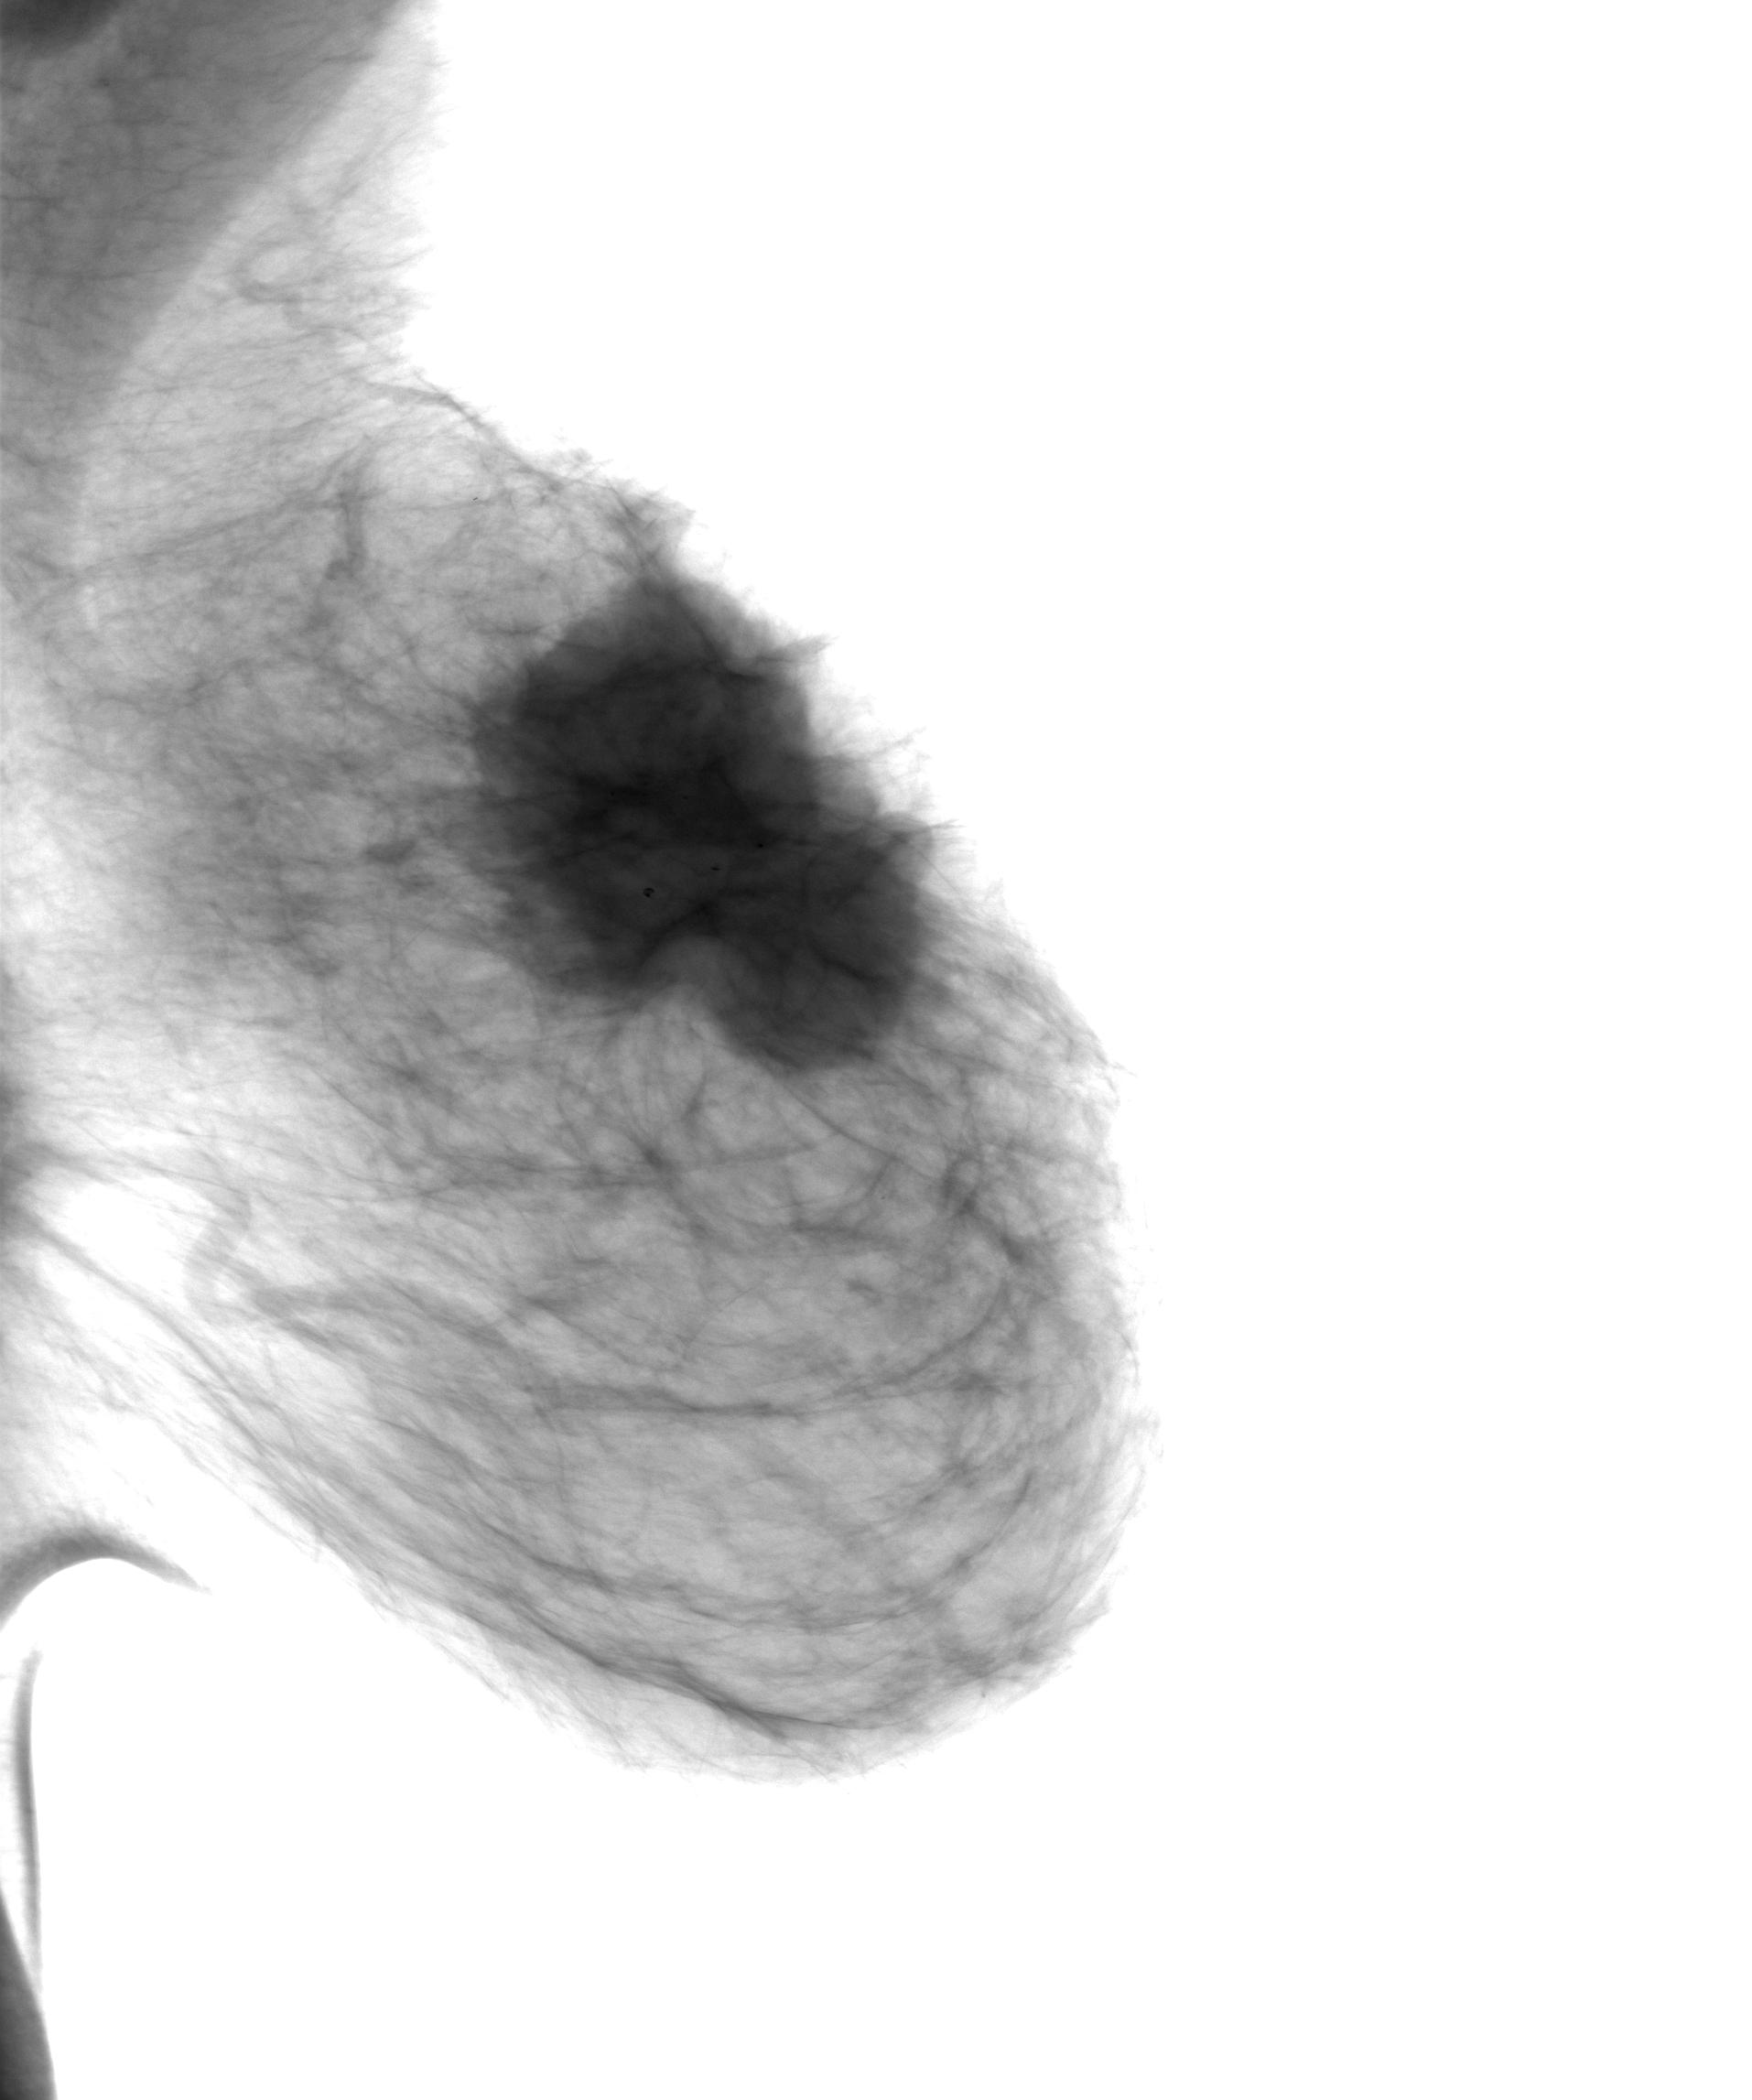
\includegraphics[width=.7\linewidth]{cancer.jpg}
  \caption{Cancer present.}
  \label{fig:sub1}
\end{subfigure}%
\begin{subfigure}{.5\textwidth}
  \centering
  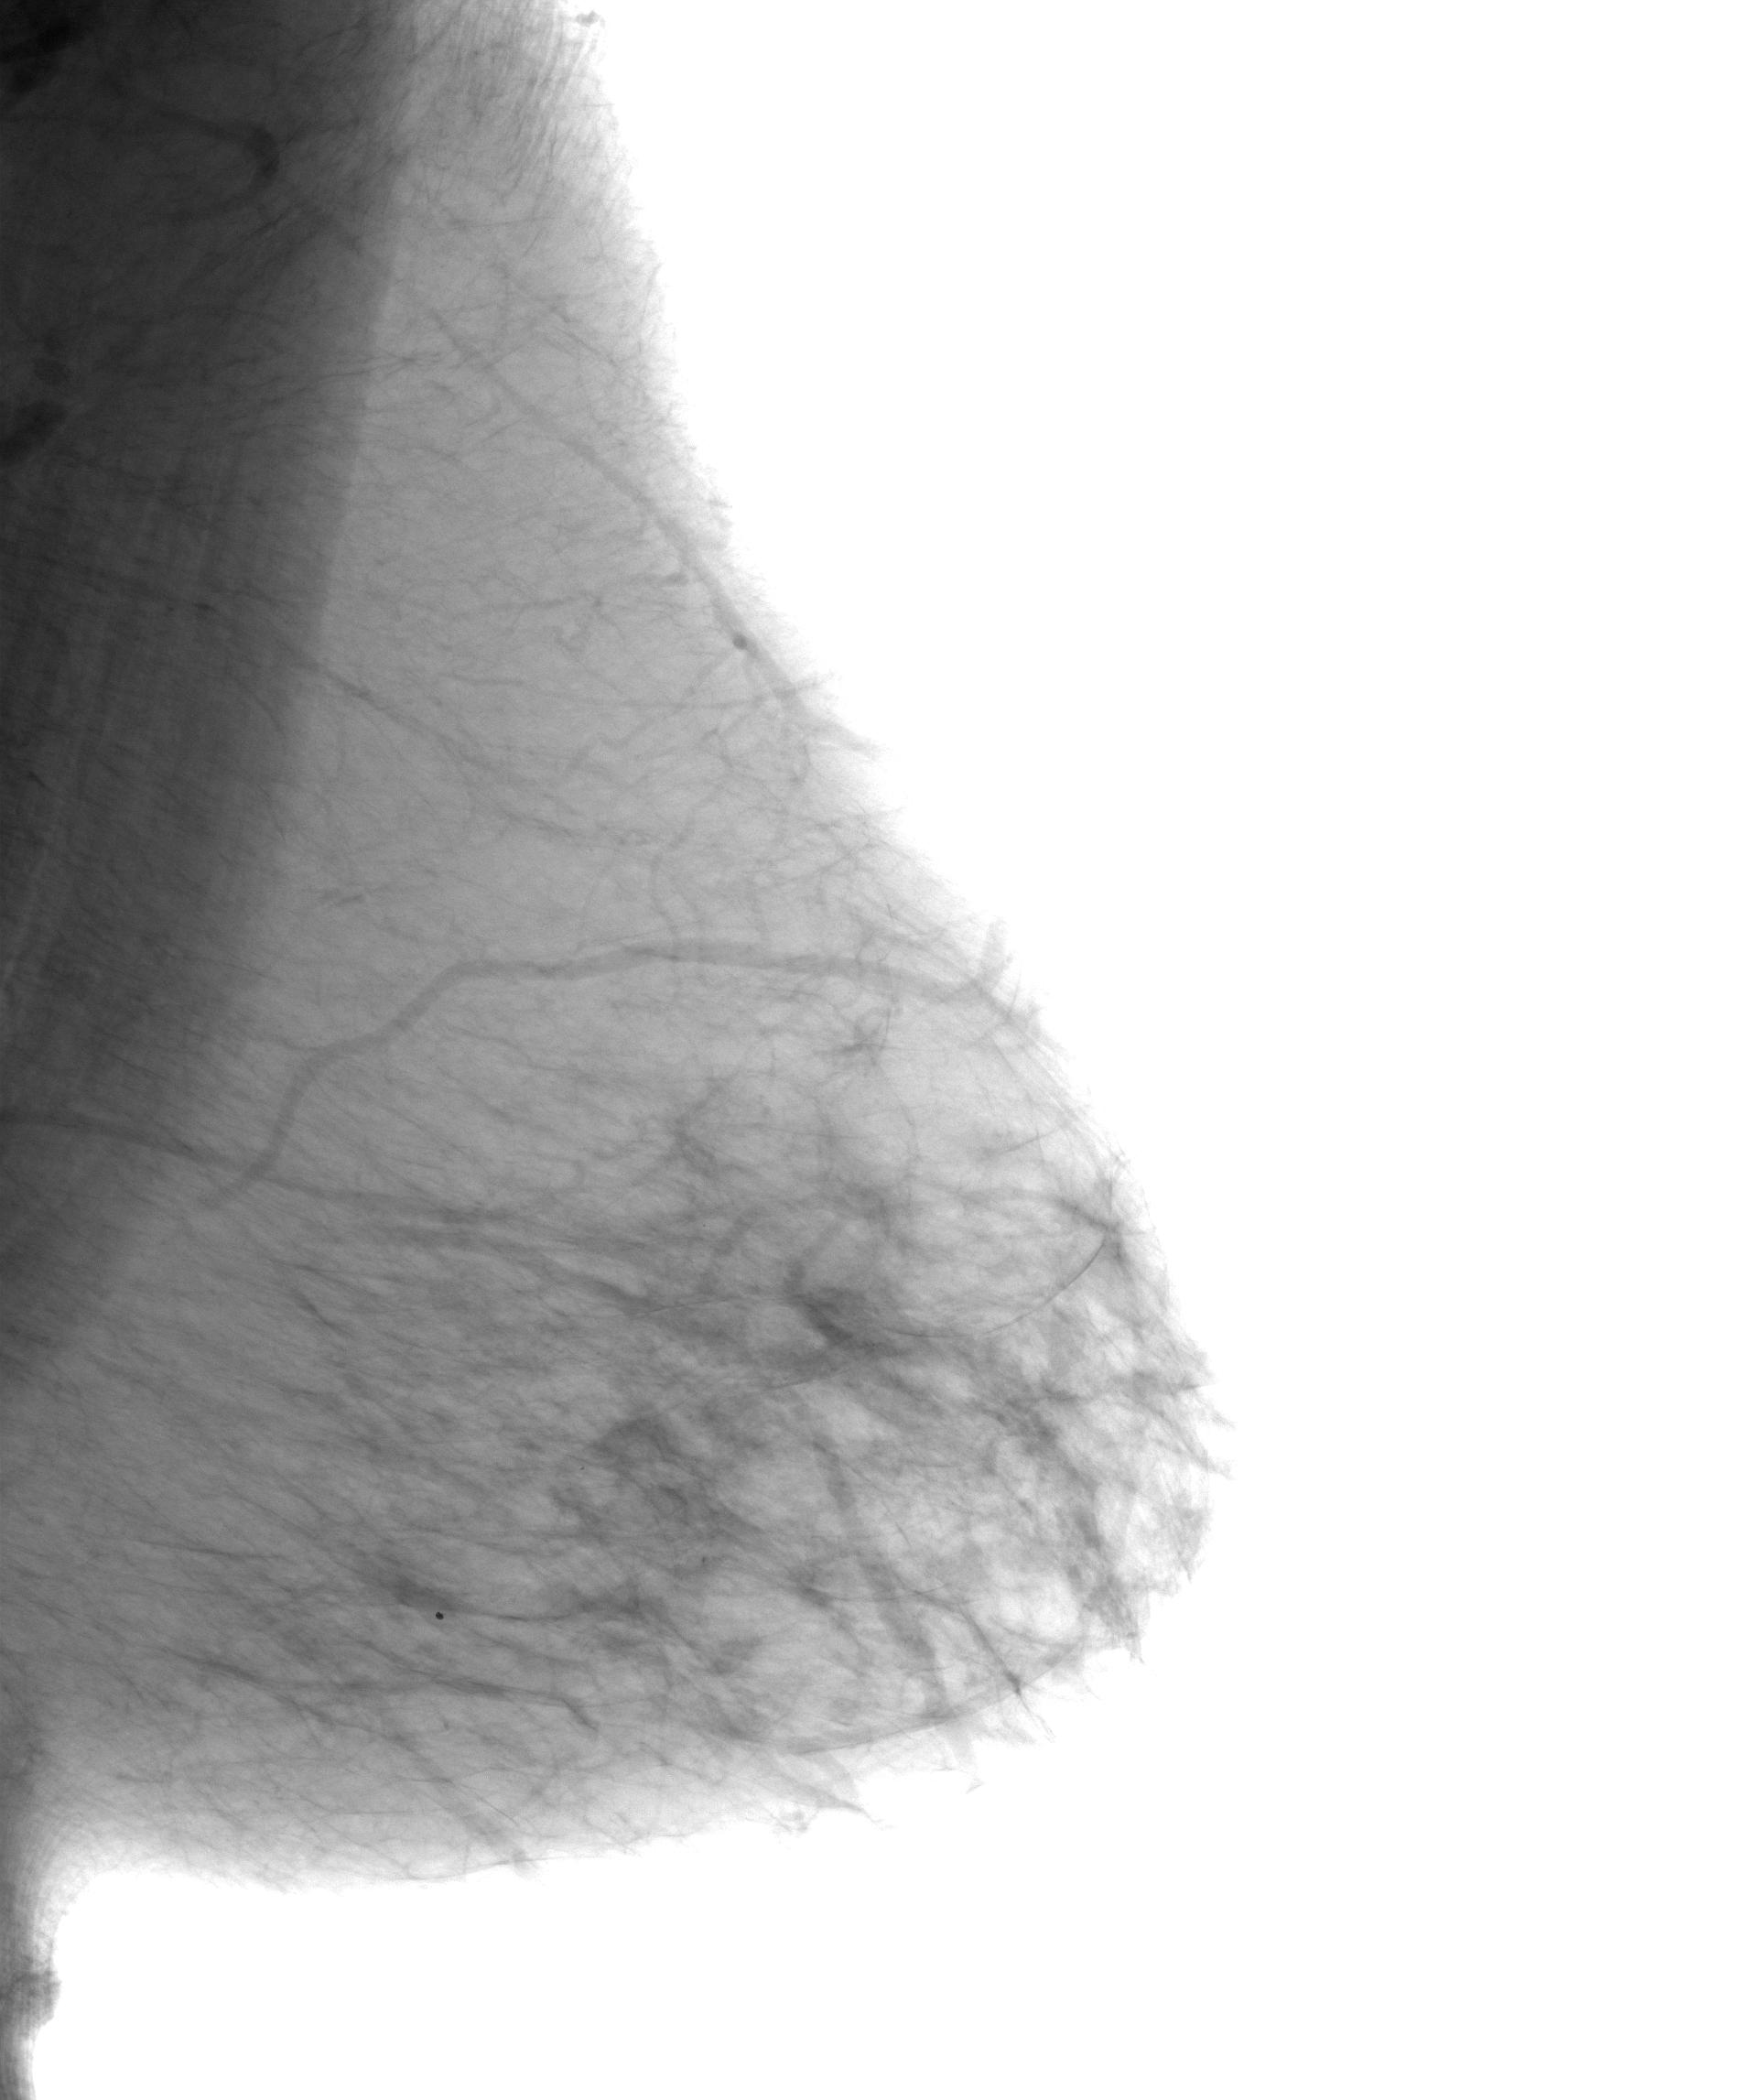
\includegraphics[width=.7\linewidth]{noCancer.jpg}
  \caption{Healthy tissue - no cancer}
  \label{fig:sub2}
\end{subfigure}
\caption{Example of the full image mammograms.  The original DICOM images were 13 bit and these have had the contrast windowed to 8 bit so that they can be printed and displayed on conventional monitors.}
\label{fig:test}
\end{figure}
\FloatBarrier
\section{Conclusions}

\newpage
%\bibliography{mybib}{}
%\bibliographystyle{plainnat}
\printbibliography

\end{document}